\pdfminorversion=4
\documentclass[aspectratio=169]{beamer}

\mode<presentation>
{
  \usetheme{default}
  \usecolortheme{default}
  \usefonttheme{default}
  \setbeamertemplate{navigation symbols}{}
  \setbeamertemplate{caption}[numbered]
  \setbeamertemplate{footline}[frame number]  % or "page number"
  \setbeamercolor{frametitle}{fg=white}
  \setbeamercolor{footline}{fg=black}
} 

\usepackage[english]{babel}
\usepackage[utf8x]{inputenc}
\usepackage{tikz}
\usepackage{courier}
\usepackage{array}
\usepackage{bold-extra}
\usepackage{minted}
\usepackage[thicklines]{cancel}
\usepackage{fancyvrb}

\xdefinecolor{dianablue}{rgb}{0.18,0.24,0.31}
\xdefinecolor{darkblue}{rgb}{0.1,0.1,0.7}
\xdefinecolor{darkgreen}{rgb}{0,0.5,0}
\xdefinecolor{darkgrey}{rgb}{0.35,0.35,0.35}
\xdefinecolor{darkorange}{rgb}{0.8,0.5,0}
\xdefinecolor{darkred}{rgb}{0.7,0,0}
\definecolor{darkgreen}{rgb}{0,0.6,0}
\definecolor{mauve}{rgb}{0.58,0,0.82}

\title[2021-05-04-hllhc-workshop]{Python Data Science}
\author{Jim Pivarski}
\institute{Princeton University -- IRIS-HEP}
\date{May the 4$^{\mbox{\scriptsize th}}$ be with you}

\usetikzlibrary{shapes.callouts}

\begin{document}

\logo{\pgfputat{\pgfxy(0.11, 7.4)}{\pgfbox[right,base]{\tikz{\filldraw[fill=dianablue, draw=none] (0 cm, 0 cm) rectangle (50 cm, 1 cm);}\mbox{\hspace{-8 cm}
\includegraphics[height=1 cm]{princeton-logo-long.png}\hspace{0.1 cm}\raisebox{0.1 cm}{
\includegraphics[height=0.8 cm]{iris-hep-logo-long.png}}\hspace{0.1 cm}}}}}

\begin{frame}
  \titlepage
\end{frame}

\logo{\pgfputat{\pgfxy(0.11, 7.4)}{\pgfbox[right,base]{\tikz{\filldraw[fill=dianablue, draw=none] (0 cm, 0 cm) rectangle (50 cm, 1 cm);}\mbox{\hspace{-8 cm}
\includegraphics[height=1 cm]{princeton-logo.png}\hspace{0.1 cm}\raisebox{0.1 cm}{
\includegraphics[height=0.8 cm]{iris-hep-logo.png}}\hspace{0.1 cm}}}}}

% Uncomment these lines for an automatically generated outline.
%\begin{frame}{Outline}
%  \tableofcontents
%\end{frame}

% START START START START START START START START START START START START START

\begin{frame}{Pythonic data analysis in the HL-LHC era?}
\vspace{0.25 cm}
\begin{center}
\only<1>{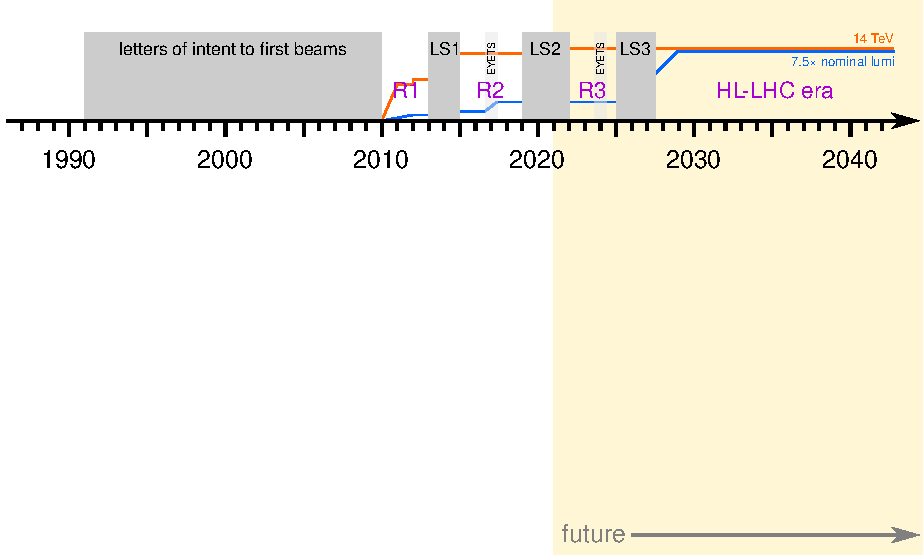
\includegraphics[width=0.9\linewidth]{hllhc-python-timeline-0.pdf}}\only<2>{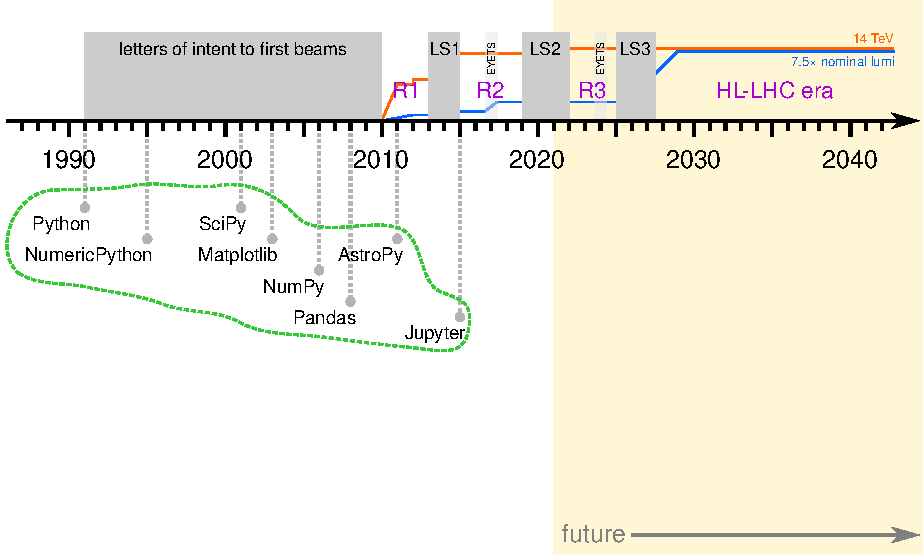
\includegraphics[width=0.9\linewidth]{hllhc-python-timeline-1.pdf}}\only<3>{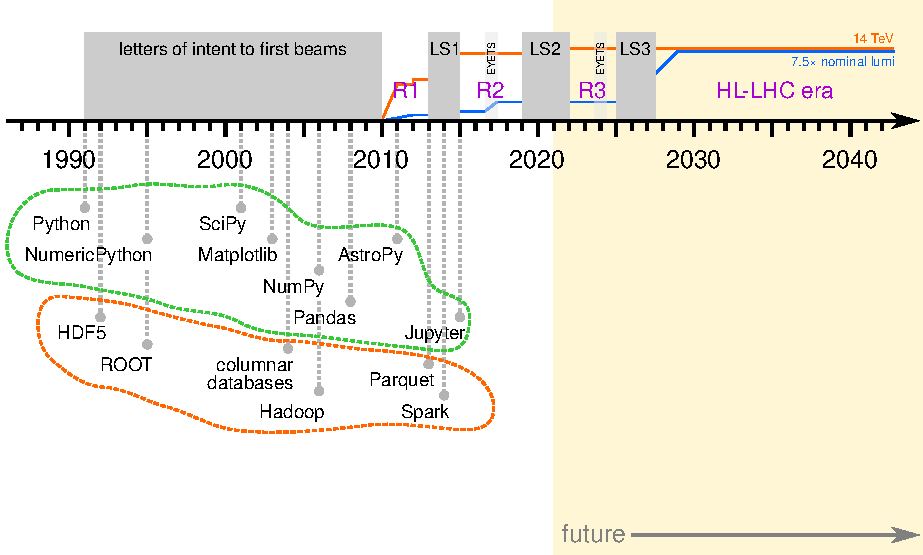
\includegraphics[width=0.9\linewidth]{hllhc-python-timeline-2.pdf}}\only<4>{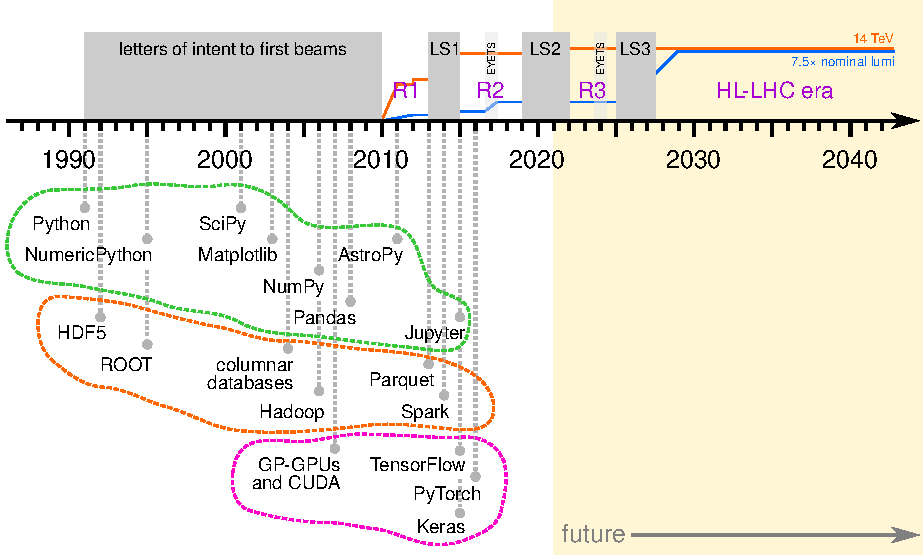
\includegraphics[width=0.9\linewidth]{hllhc-python-timeline-3.pdf}}\only<5>{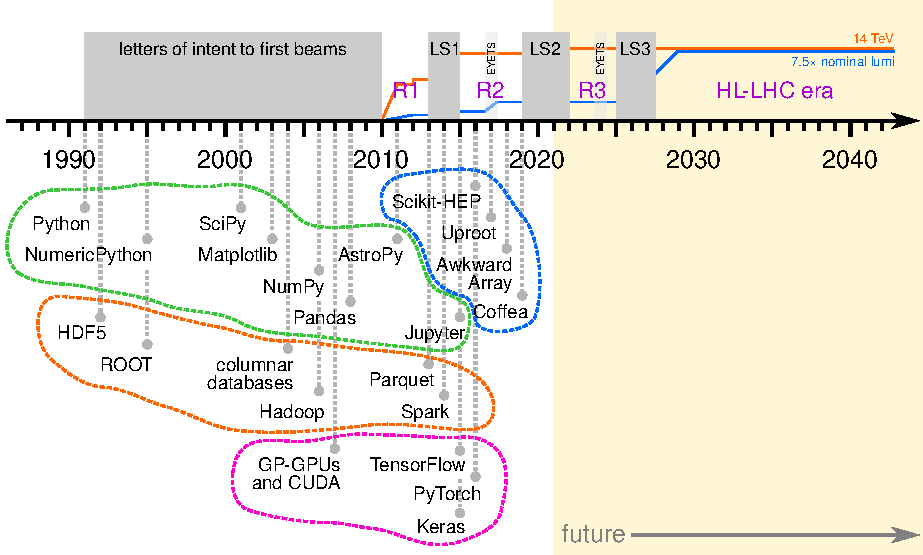
\includegraphics[width=0.9\linewidth]{hllhc-python-timeline-4.pdf}}\only<6>{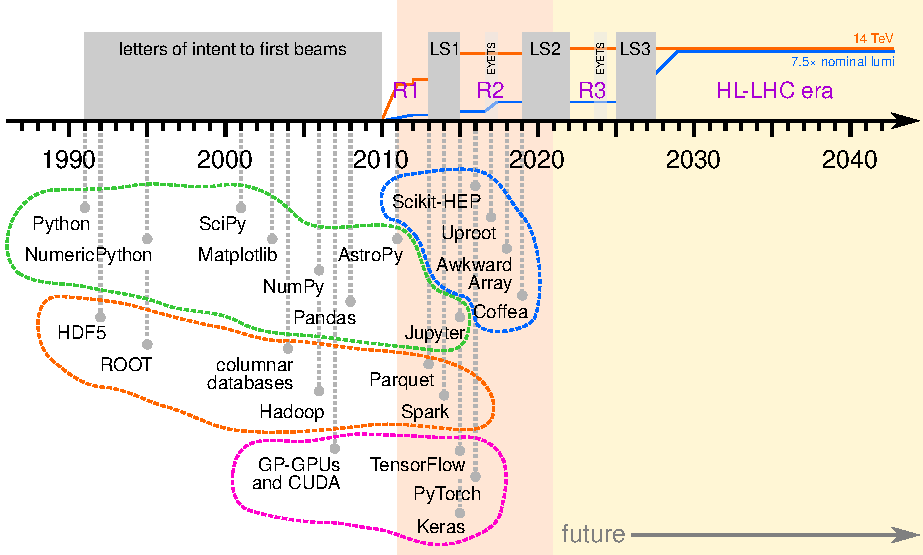
\includegraphics[width=0.9\linewidth]{hllhc-python-timeline-5.pdf}}
\end{center}
\end{frame}

\begin{frame}{Physicists have been moving to Python on their own}
\vspace{0.35 cm}

Primary language of GitHub repos created by users who forked CMSSW:

\vspace{-0.6 cm}
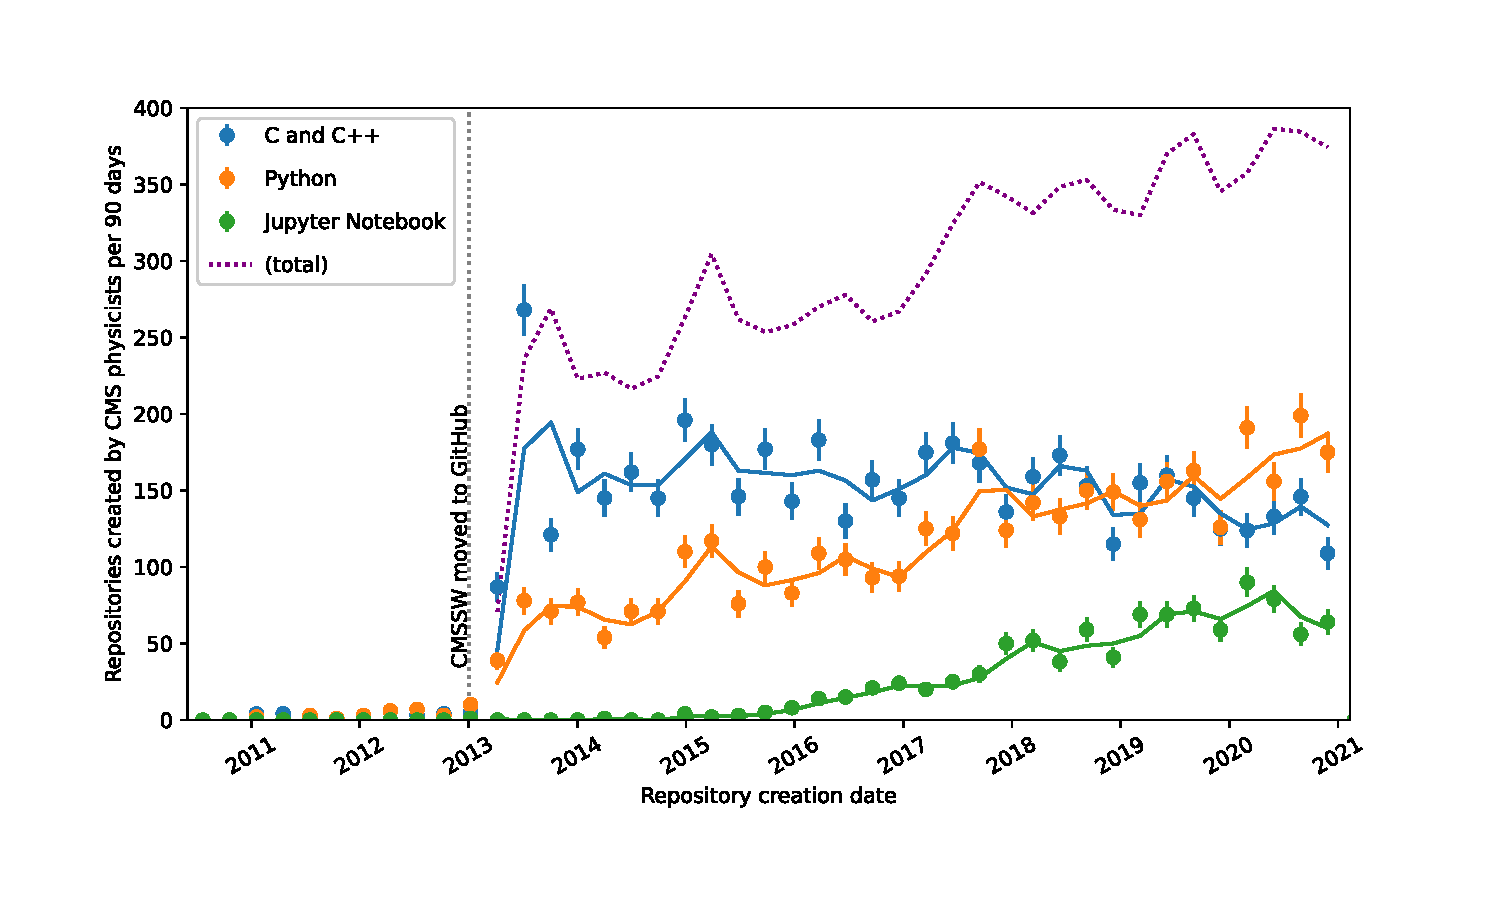
\includegraphics[width=\linewidth]{lhlhc-github-languages.pdf}
\end{frame}

\begin{frame}{Consistent with survey results (PyHEP 2020 participants)}
\vspace{0.2 cm}
\begin{columns}
\column{1.15\linewidth}
\only<1>{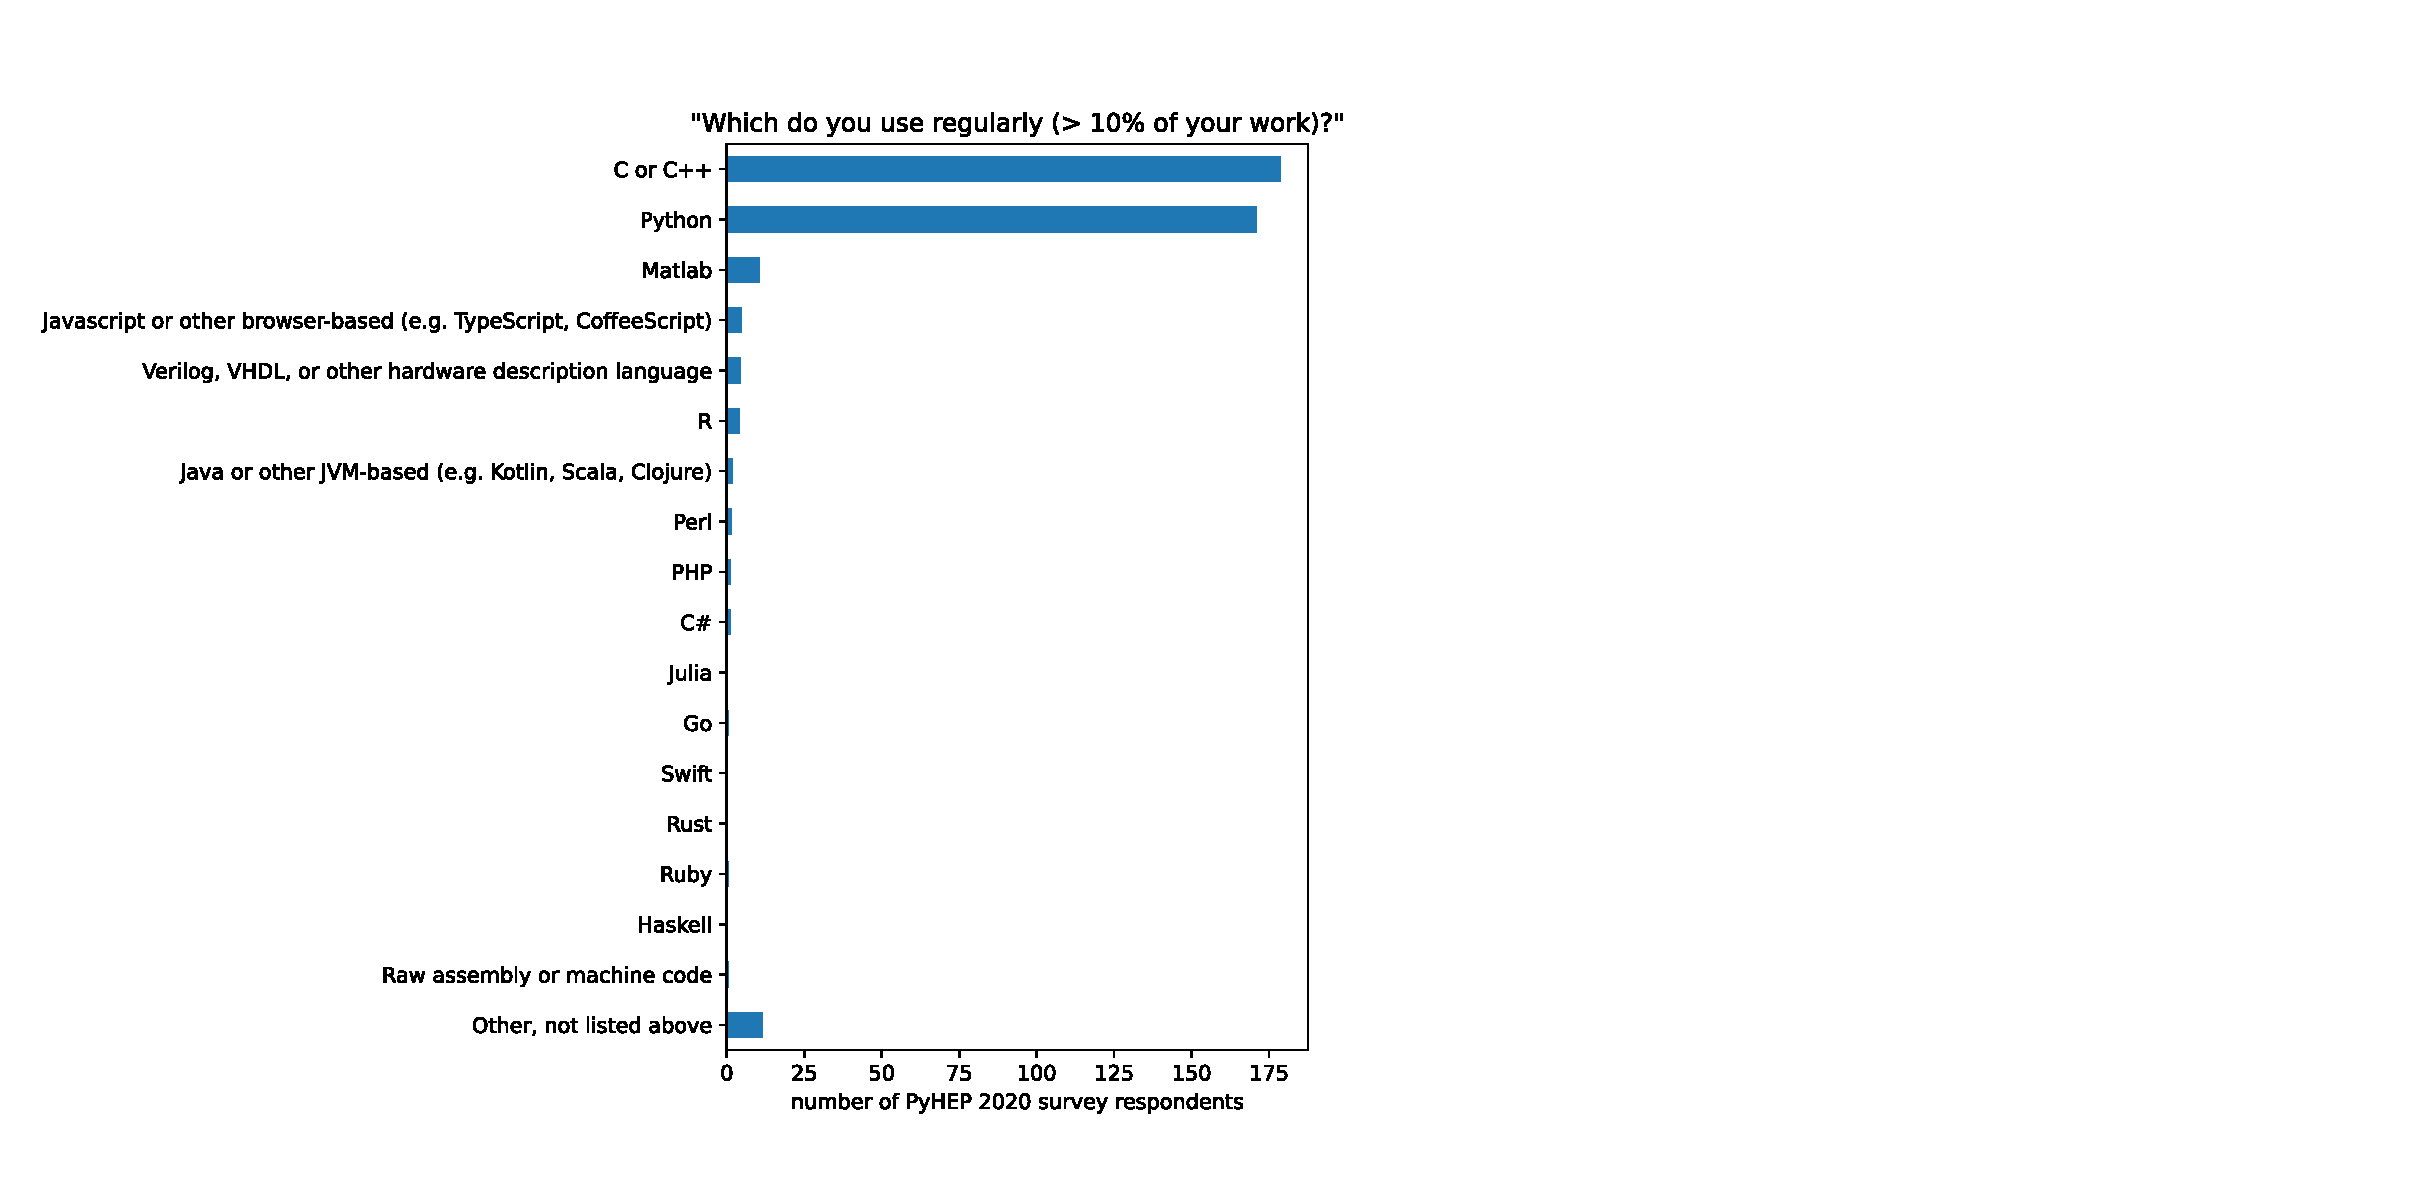
\includegraphics[width=\linewidth]{pyhep2020-survey-1.pdf}}\only<2>{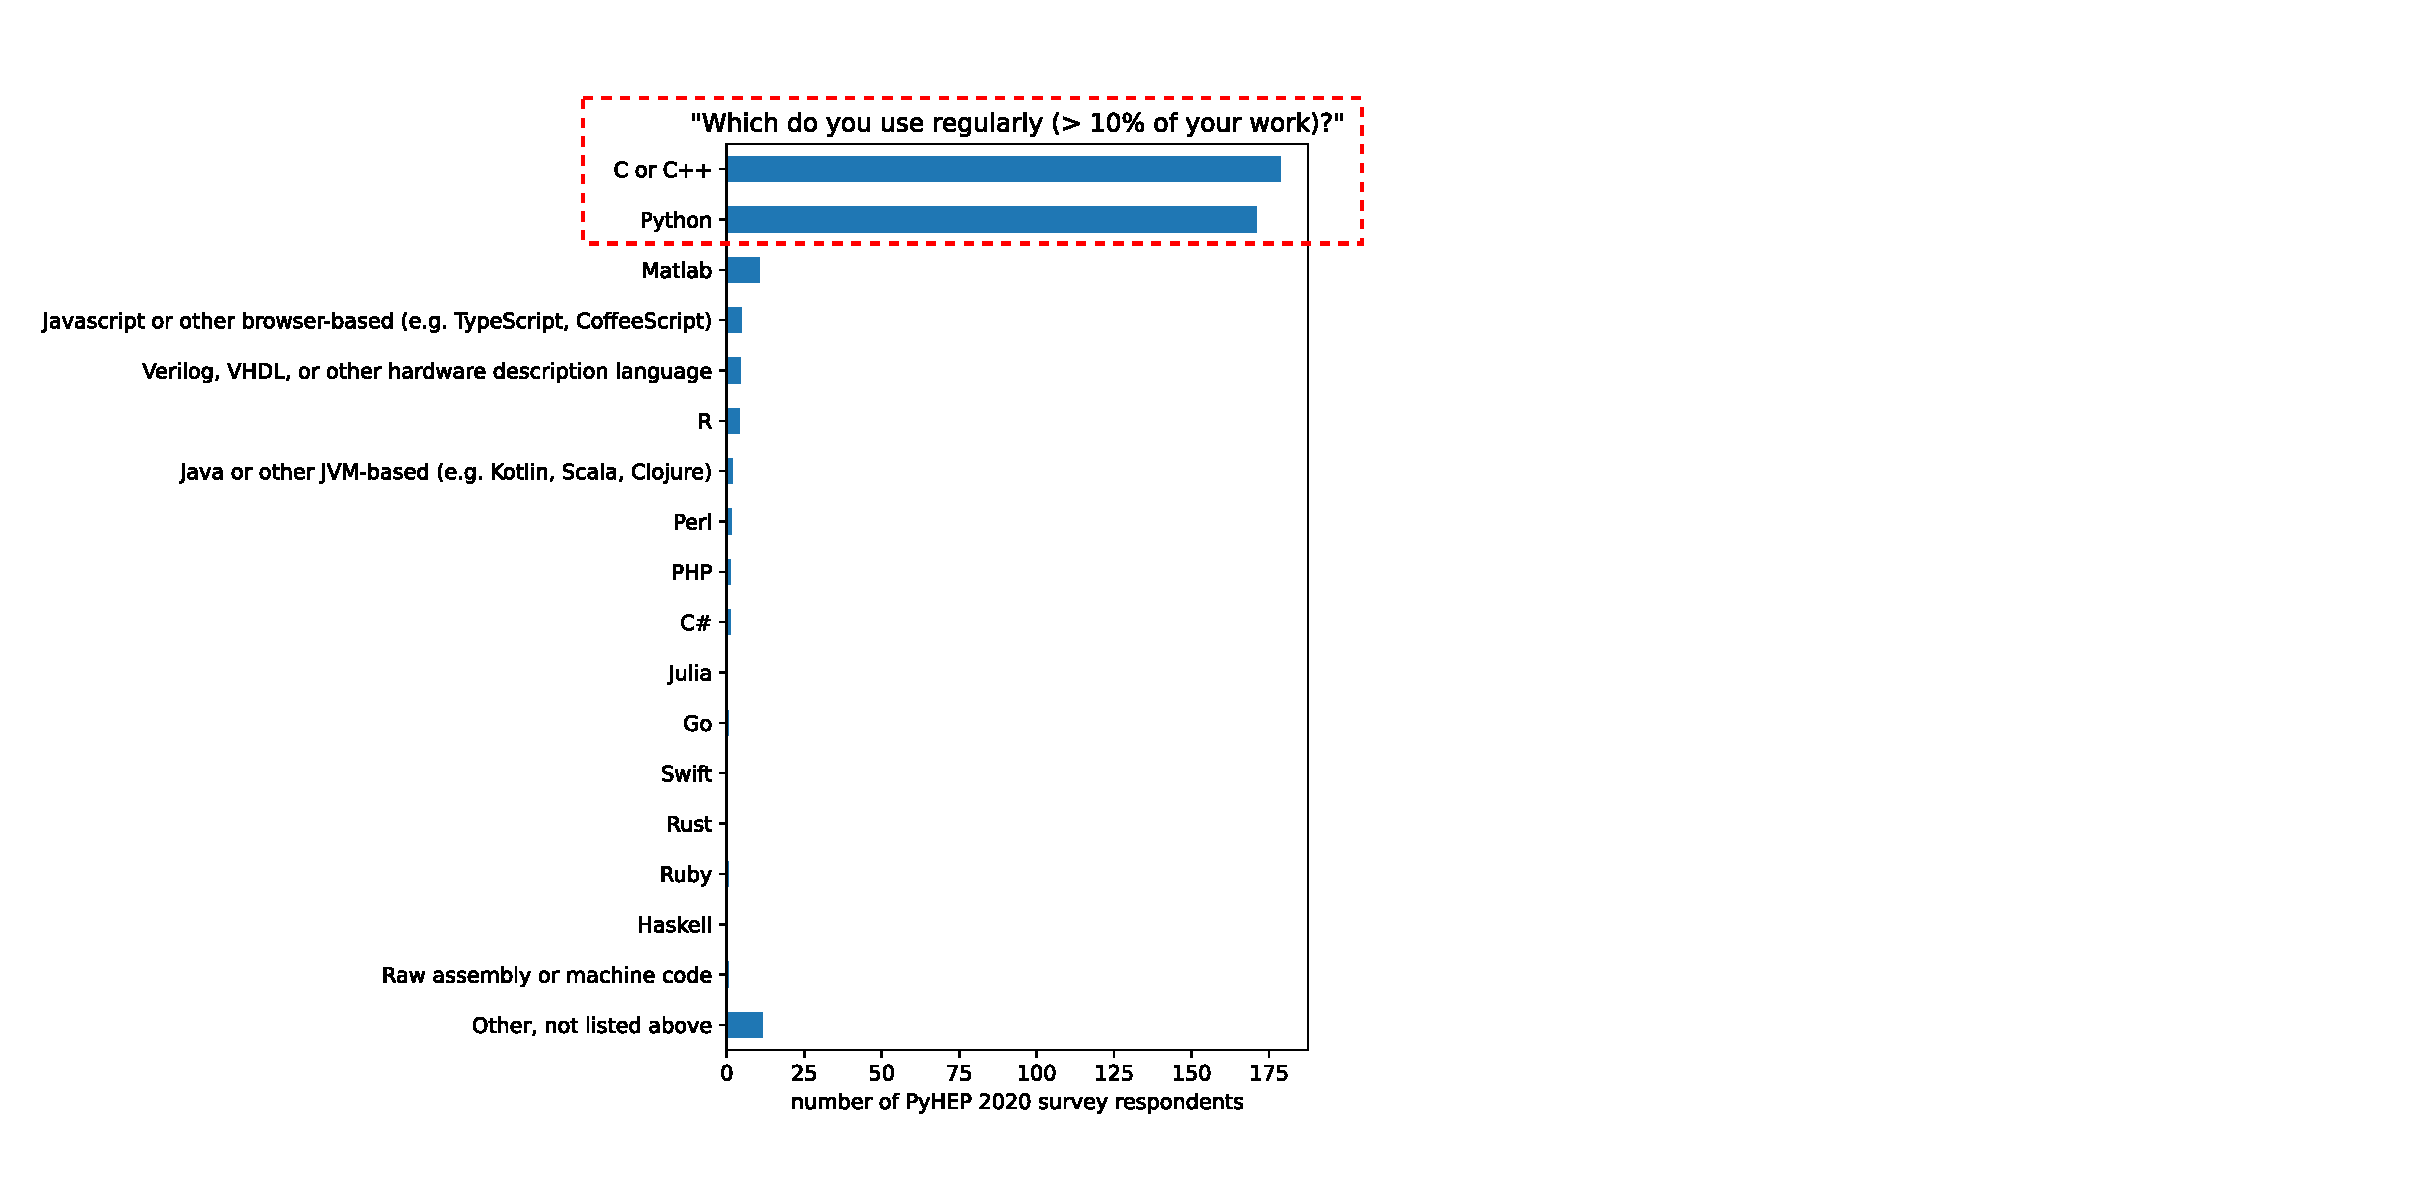
\includegraphics[width=\linewidth]{pyhep2020-survey-2.pdf}}\only<3>{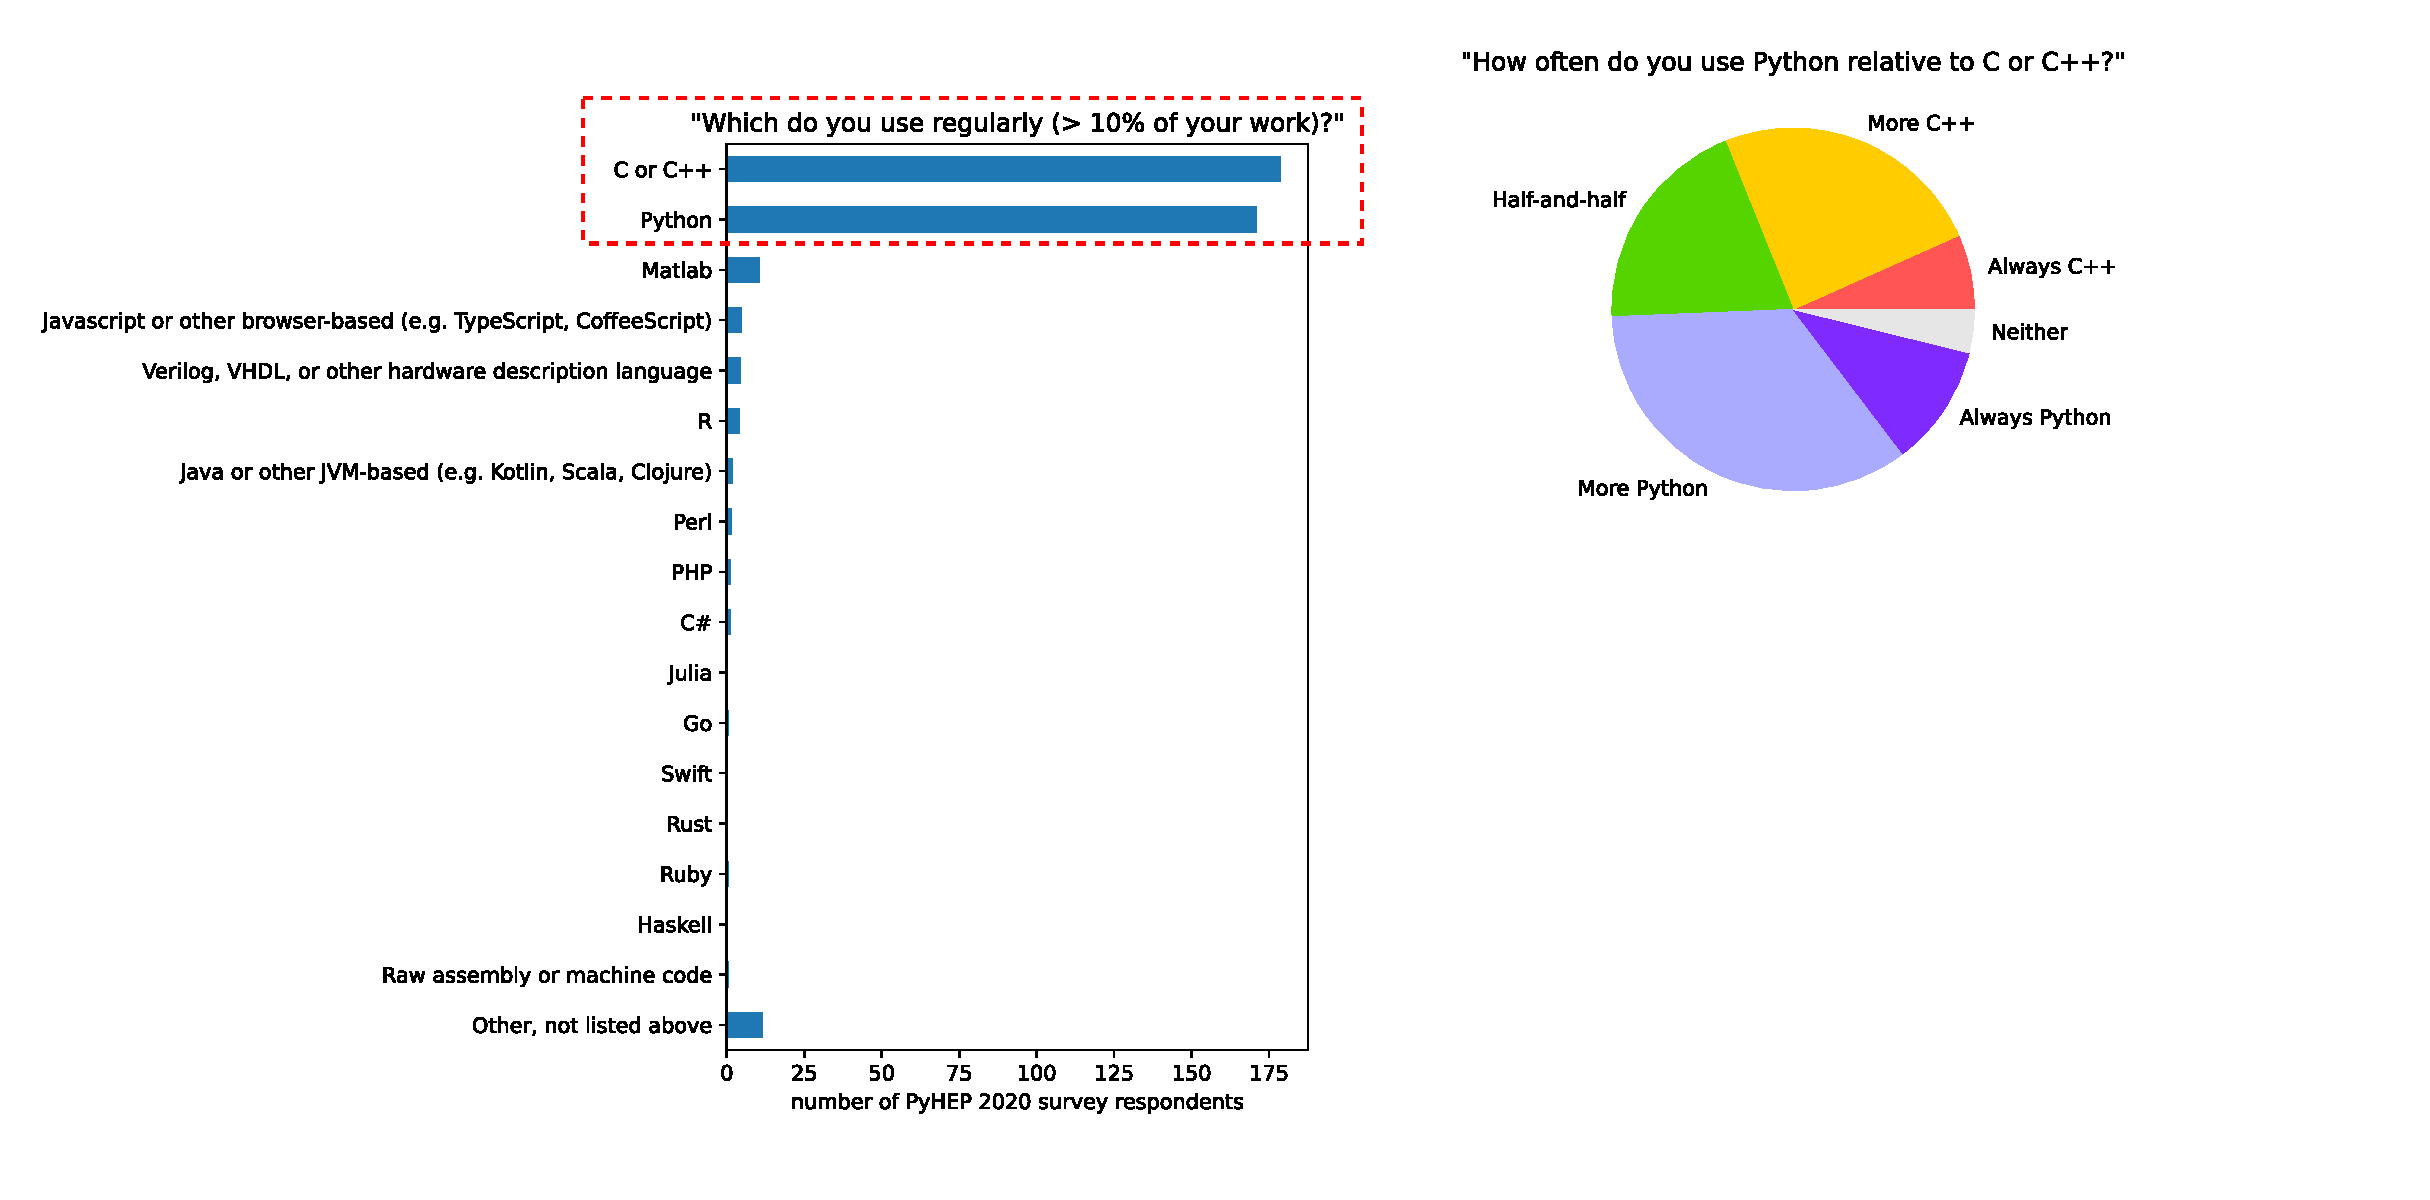
\includegraphics[width=\linewidth]{pyhep2020-survey-3.pdf}}\only<4>{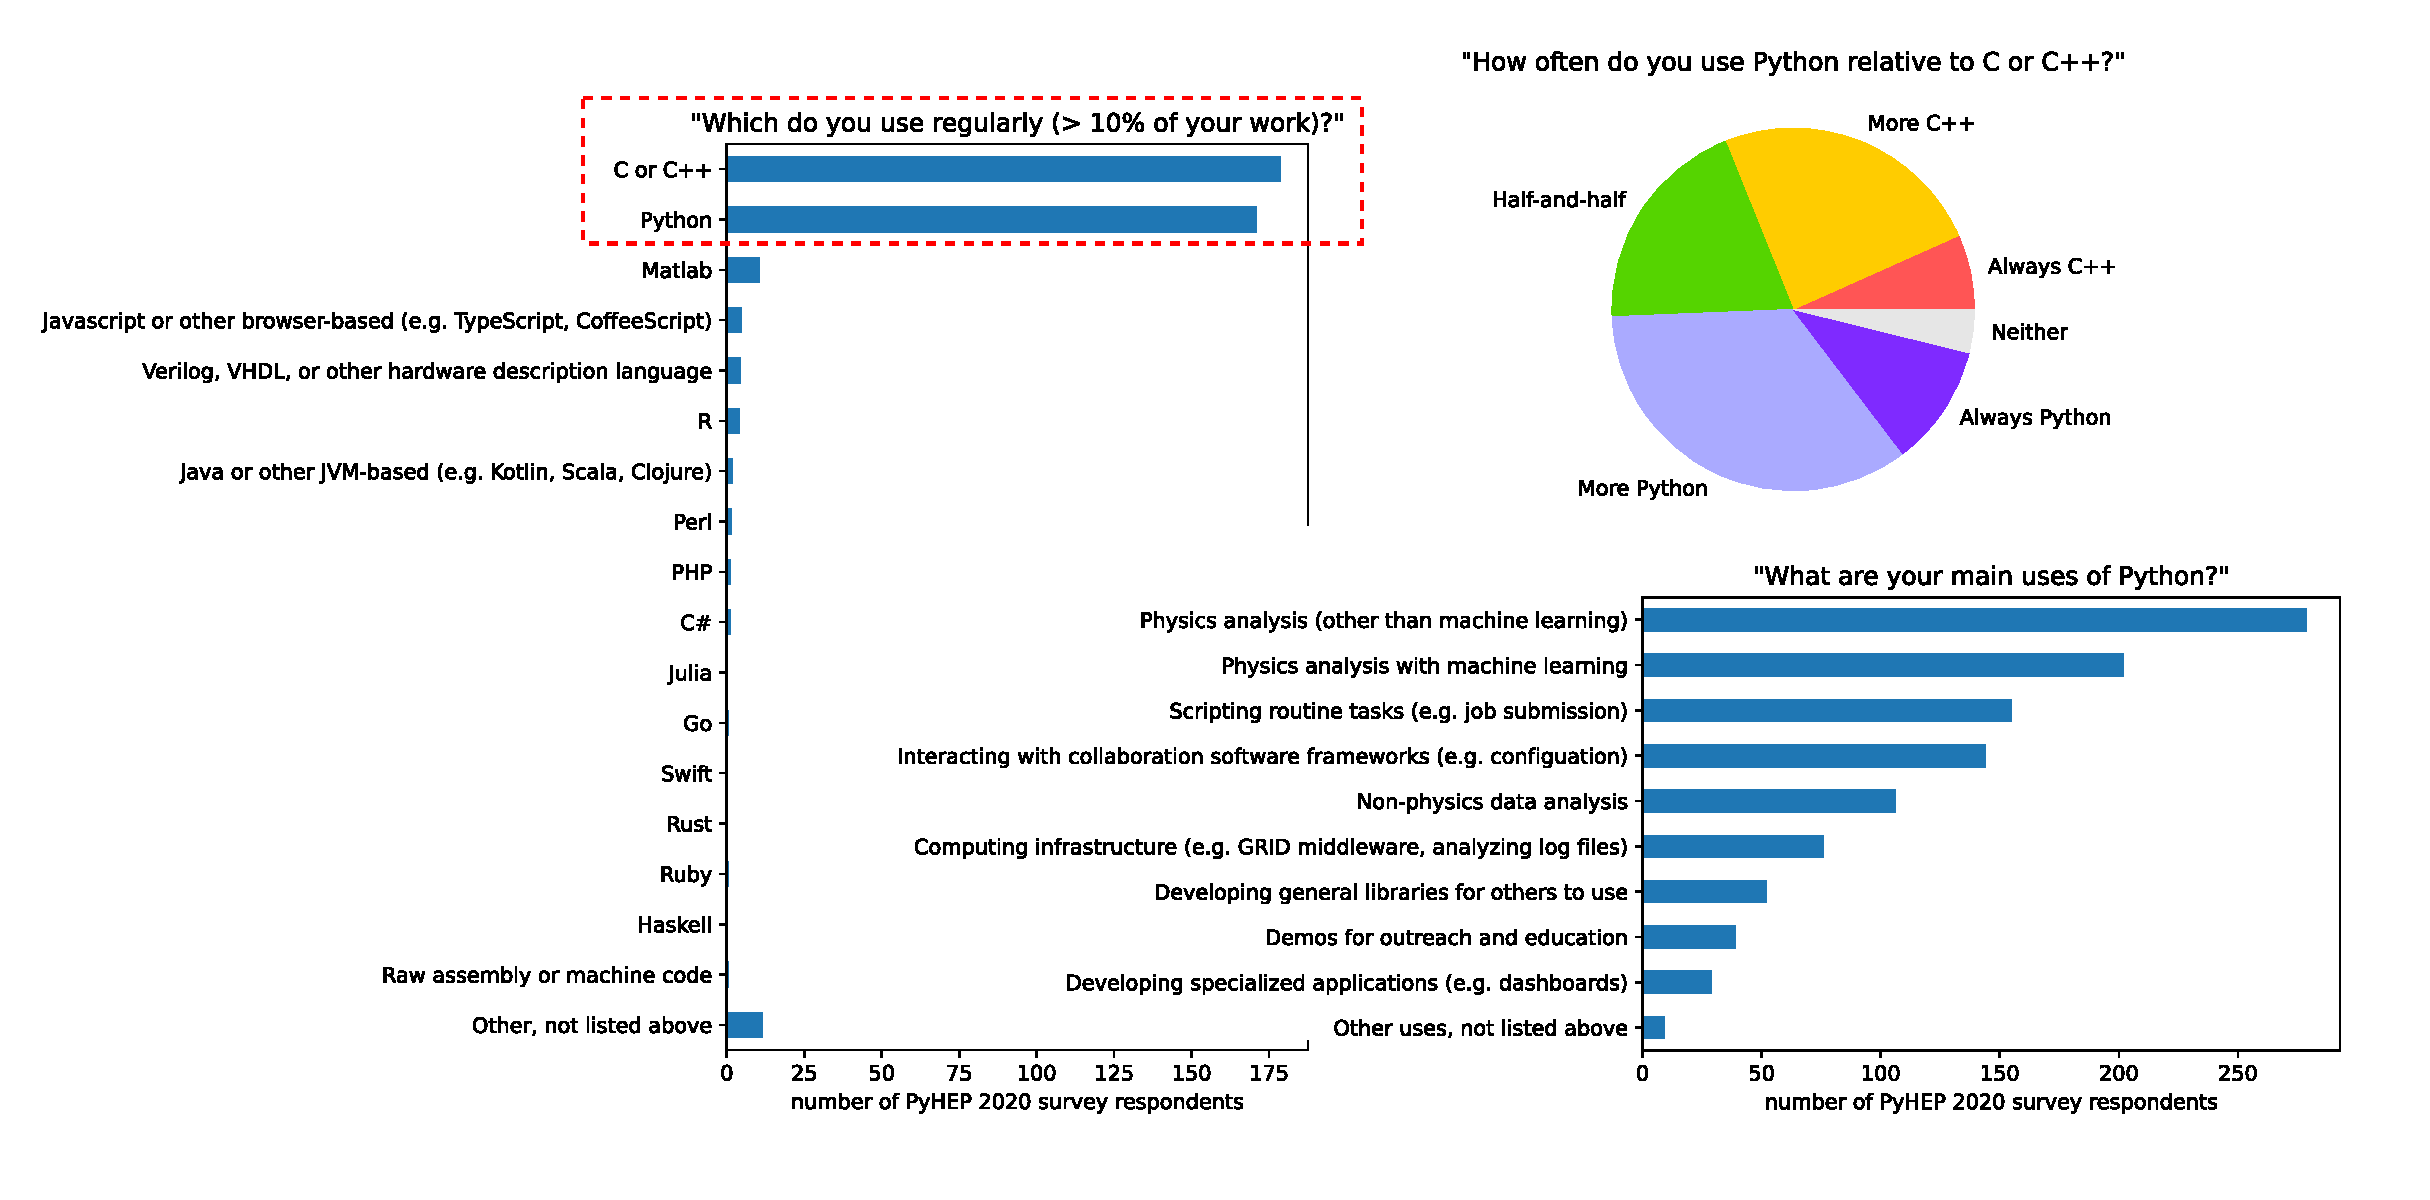
\includegraphics[width=\linewidth]{pyhep2020-survey-4.pdf}}\only<5>{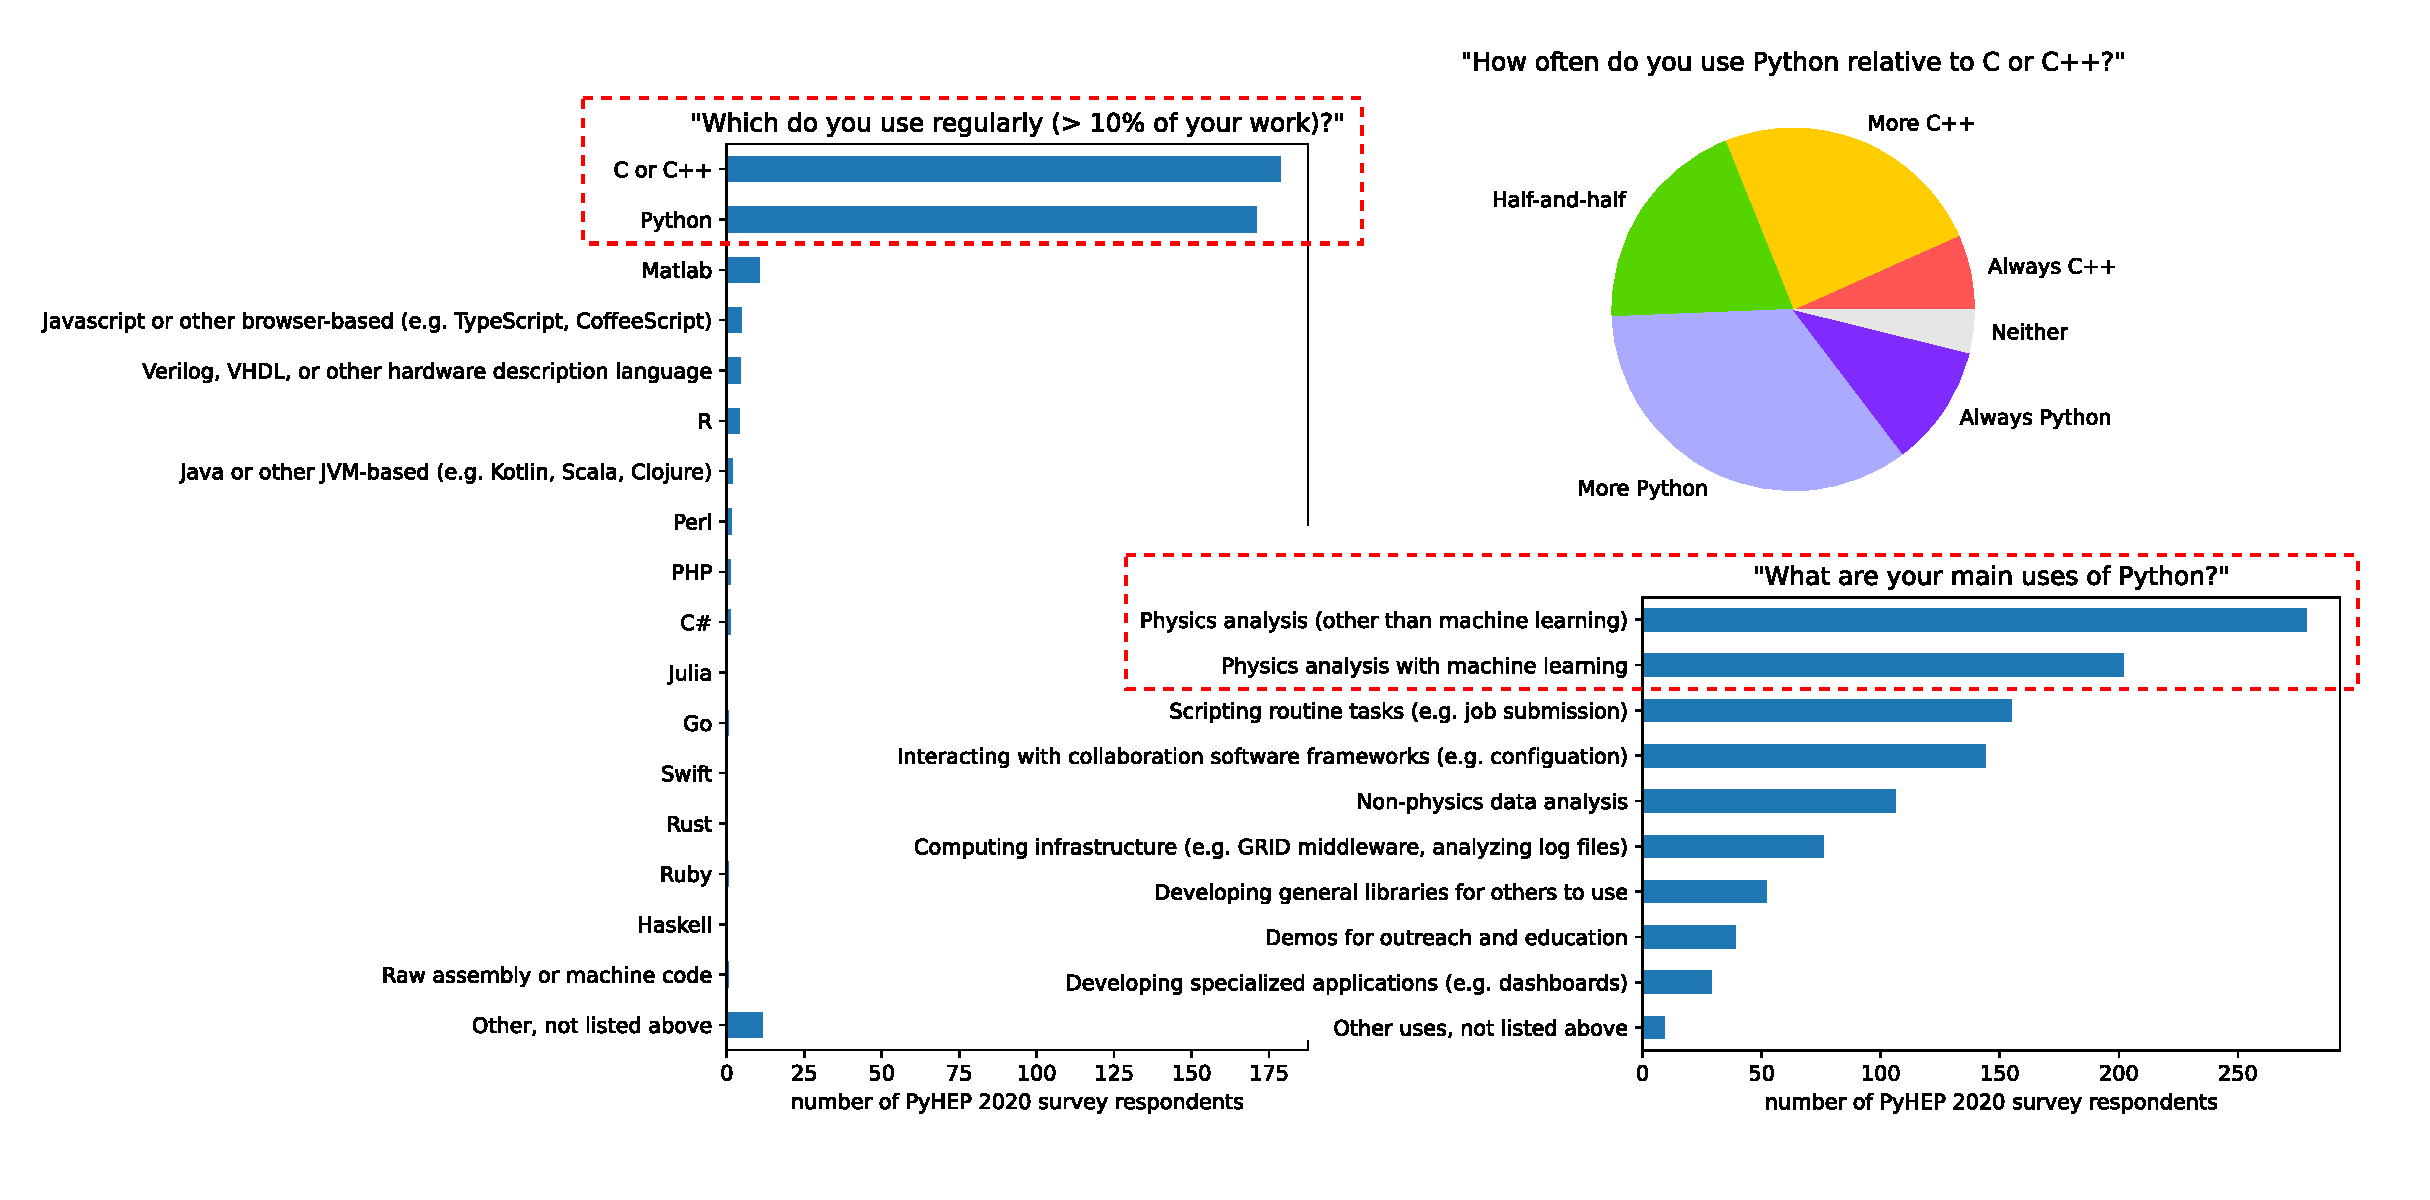
\includegraphics[width=\linewidth]{pyhep2020-survey-5.pdf}}
\end{columns}
\end{frame}

\begin{frame}{Pythonic analysis is mainstream; trend preceded Uproot}
\vspace{0.35 cm}

GitHub repos matching search strings: Pythonic analysis is as common as ``TFile''.

\vspace{-0.6 cm}
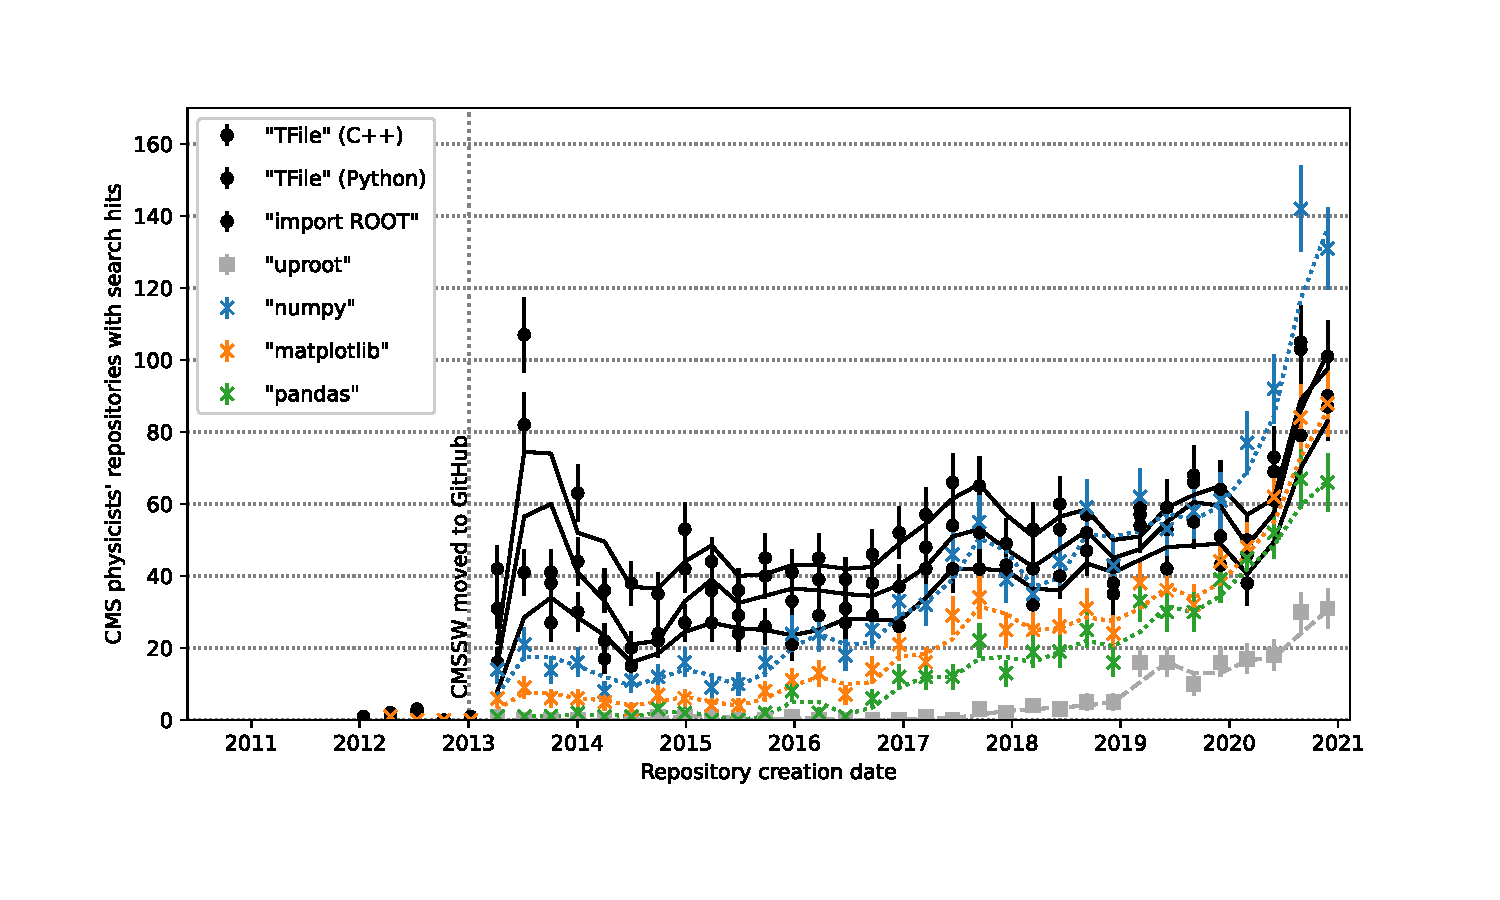
\includegraphics[width=\linewidth]{lhlhc-github-overlay-lin.pdf}
\end{frame}

\begin{frame}{This is also consistent with self-reported usage}
\vspace{-0.35 cm}
\begin{columns}
\column{1.1\linewidth}
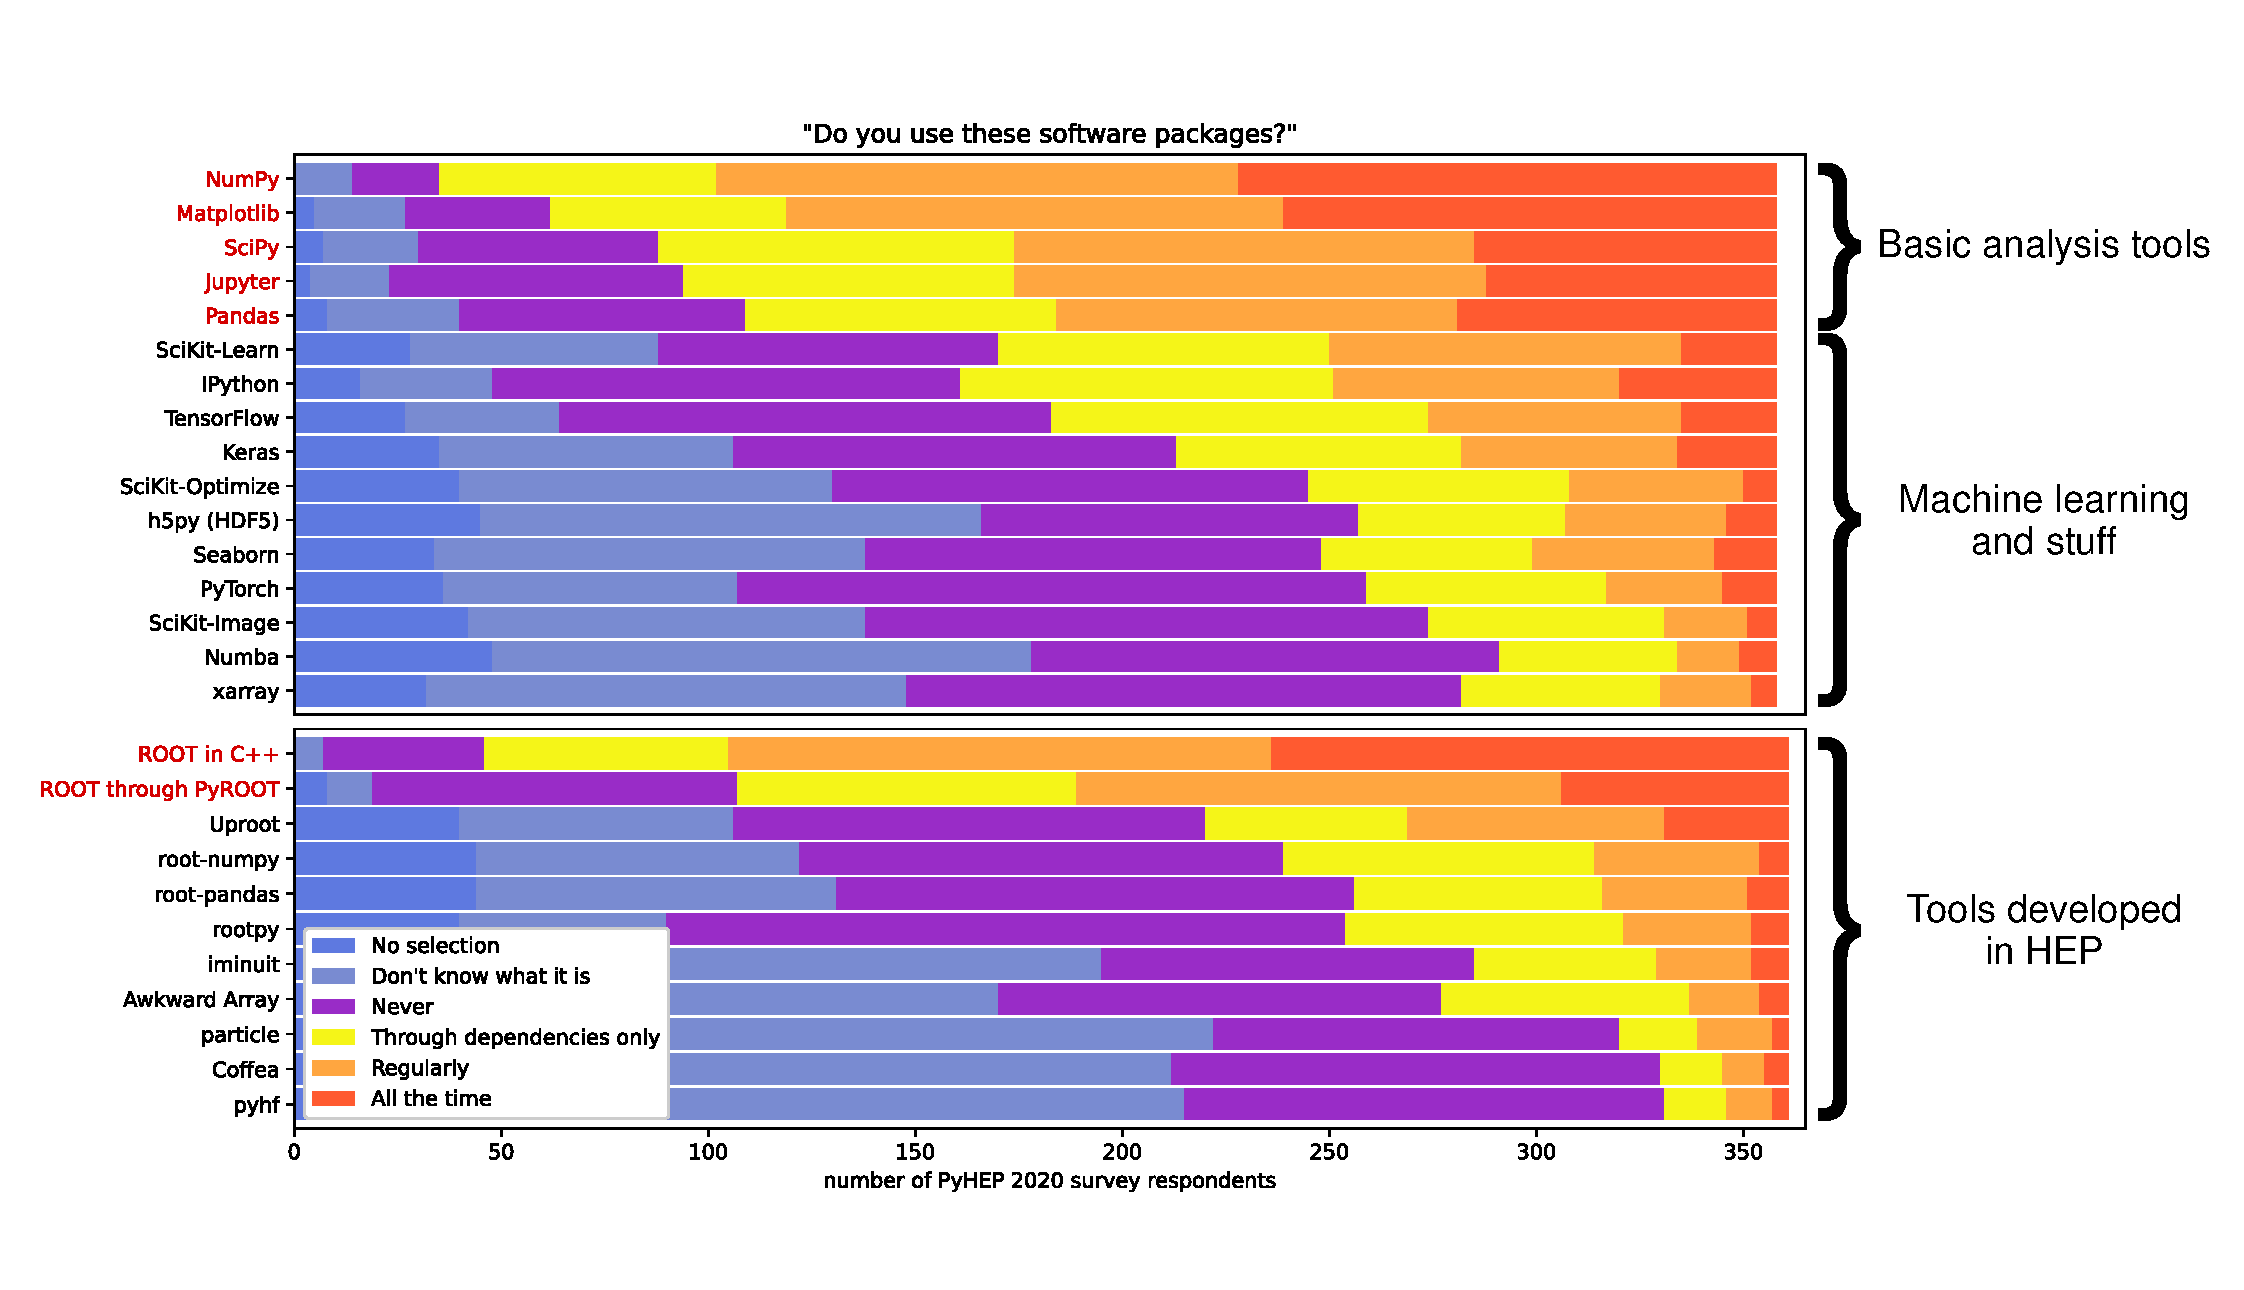
\includegraphics[width=\linewidth]{lhlhc-familiarity-with-packages.pdf}
\end{columns}
\end{frame}

\end{document}
